
\def\dX{3.0}
\def\dY{3.0}
\def\dR{0.7}

  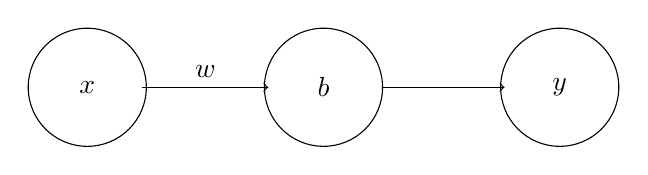
\begin{tikzpicture}
    %%   (lable)  (x, y)     {\text}
    \coordinate (CX1) at (-\dX+\dR,         0);
    \coordinate (CN1) at (    -\dR,         0);
    \coordinate (CY)  at ( \dX-\dR,         0);

    \node[shape=circle,draw=black, minimum size=1.5cm] (X1) at (-\dX,  0) {$x$};
    \node[shape=circle,draw=black, minimum size=1.5cm] (N1) at (0,     0) {$b$};
    \node[shape=circle,draw=black, minimum size=1.5cm] (Y)  at (+\dX,  0) {$y$};

    \path[->] (CX1) edge node[above] {$w$} (CN1);
    \path[->] (N1) edge (CY);

  \end{tikzpicture}
